\lecture{Crittografia}{31~-~01~-~2026}
%
%
\section{Fondamenti di Crittografia Applicata}
La crittografia è definita come la ``scienza della scrittura segreta''. Il processo fondamentale coinvolge la trasformazione di un messaggio leggibile, chiamato \emph{plain text}, in un messaggio incomprensibile, chiamato \emph{cipher text}, tramite un algoritmo di cifratura e una sua chiave. Per recuperare il messaggio originale, il ricevente utilizza un algoritmo di decifratura insieme alla sua chiave.

I dati da proteggere possono trovarsi in tre stati fondamentali:
\begin{itemize}
    \item \textbf{Data at rest}: Dati archiviati (es. su Hard Disk);
    \item \textbf{Data in transit}: Dati in movimento su una rete;
    \item \textbf{Data in use}: Dati in elaborazione nella RAM.
\end{itemize}

%
\section{Algoritmi Crittografici}
Gli algoritmi si dividono principalmente in simmetrici e asimmetrici. È cruciale ricordare le differenze nelle dimensioni delle chiavi e dei blocchi.
%
\subsection{Crittografia Simmetrica}
Utilizza la stessa chiave per cifrare e decifrare.
\begin{itemize}
    \item \textbf{DES}: Chiave da 56bit e blocchi da 64bit, è obsoleto;
    \item \textbf{3DES}: Utilizza una chiave a 112 bit e blocchi da 64 bit;
    \item \textbf{AES (Advanced Encryption Standard)}: Lo standard attuale. Utilizza blocchi da 128 bit e chiavi variabili da 128 a 256 bit;
    \item \textbf{ChaCha20}: È uno stream cipher (cifra bit per bit invece che a blocchi), definito nell'RFC-8439.
    \item \textbf{RC4}: Un'altro stream cipher simmetrico.
\end{itemize}

%
\subsection{Crittografia Asimmetrica}
Utilizza una coppia di chiavi (pubblica e privata).
\begin{itemize}
    \item \textbf{RSA}: Basato sulla fattorizzazione dei numeri primi. Chiavi tra 512 e 4096 bit;
    \item \textbf{DSA}: Basato sul logaritmo discreto (Standard NIST FIPS-186). Chiavi tra 512 e 3072 bit;
    \item \textbf{ECDSA}: Variante di DSA basata su curve ellittiche.
\end{itemize}

\begin{figure}
    \centering
    % Sottofigura 1: Crittografia Simmetrica (es. AES)
    \begin{subfigure}{0.45\linewidth}
        \centering
        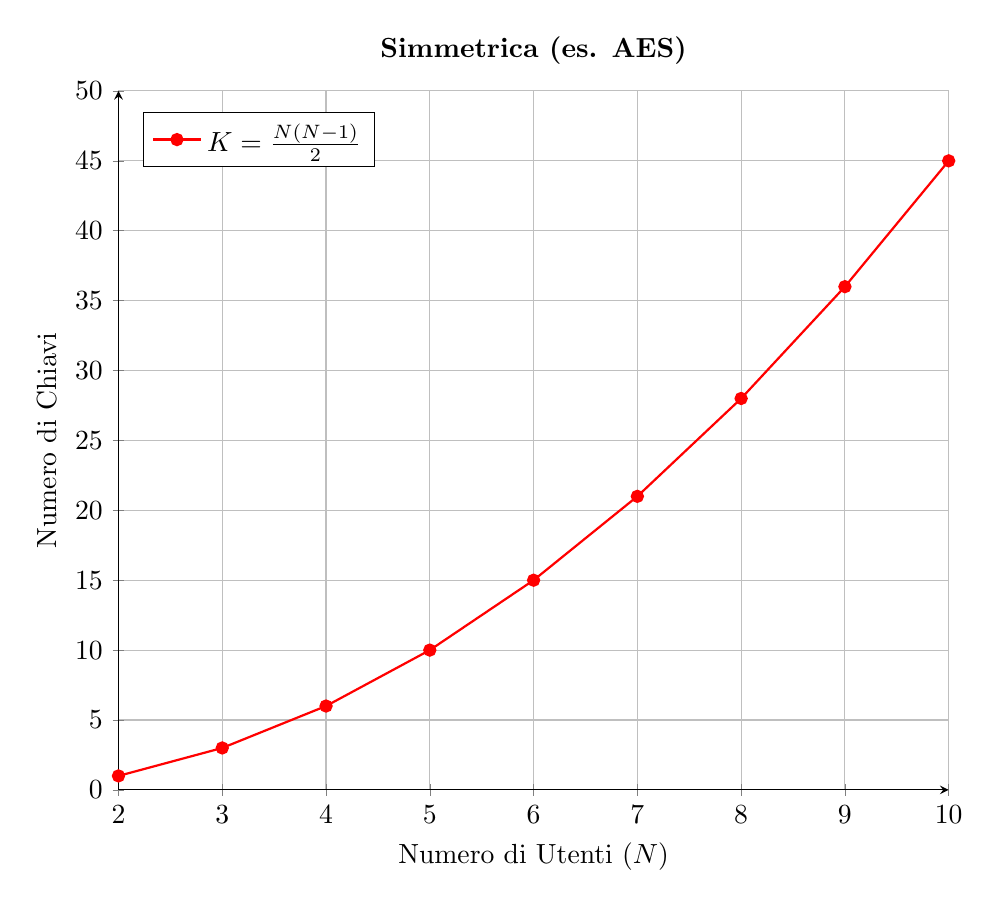
\begin{tikzpicture}
            \begin{axis}[
                    title={\textbf{Simmetrica (es. AES)}},
                    xlabel={Numero di Utenti ($N$)},
                    ylabel={Numero di Chiavi},
                    grid=major,
                    width=\linewidth,
                    xmin=2, xmax=10,
                    ymin=0, ymax=50,
                    legend pos=north west,
                    axis lines=left,
                    cycle list name=color list
                ]
                % Funzione: N*(N-1)/2
                % Dati dalla Slide 19 del PDF
                \addplot[
                    color=red,
                    mark=*,
                    thick,
                    domain=2:10,
                    samples=9
                ]
                {(x*(x-1))/2};
                \addlegendentry{$K = \frac{N(N-1)}{2}$}
            \end{axis}
        \end{tikzpicture}
        \caption{Crescita esponenziale delle chiavi (Problematicità in AES)}
        \label{fig:sym_crypto}
    \end{subfigure}
    \hfill
    % Sottofigura 2: Crittografia Asimmetrica (es. RSA)
    \begin{subfigure}{0.45\linewidth}
        \centering
        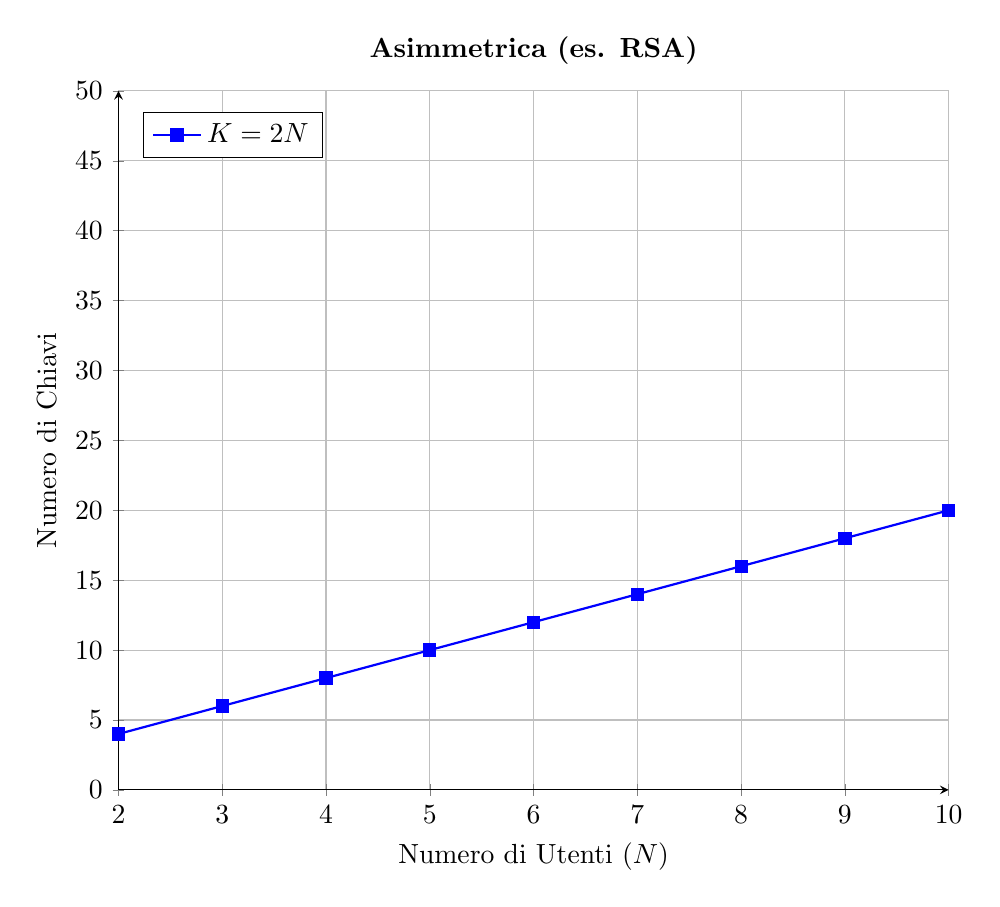
\begin{tikzpicture}
            \begin{axis}[
                    title={\textbf{Asimmetrica (es. RSA)}},
                    xlabel={Numero di Utenti ($N$)},
                    ylabel={Numero di Chiavi},
                    grid=major,
                    width=\linewidth,
                    xmin=2, xmax=10,
                    ymin=0, ymax=50,
                    legend pos=north west,
                    axis lines=left
                ]
                % Funzione: 2*N
                % Dati dalla Slide 19 del PDF
                \addplot[
                    color=blue,
                    mark=square*,
                    thick,
                    domain=2:10,
                    samples=9
                ]
                {2*x};
                \addlegendentry{$K = 2N$}
            \end{axis}
        \end{tikzpicture}
        \caption{Crescita lineare delle chiavi (Scalabilità in RSA)}
        \label{fig:asym_crypto}
    \end{subfigure}

    \caption{Confronto della complessità di gestione delle chiavi tra gli standard crittografici più diffusi}
    \label{fig:crypto_comparison}
\end{figure}

%
\subsection{Differenza nell'elaborazione dei dati}
%
\paragraph{Block Cipher (Cifrari a blocchi)} Trasformano un blocco di dimensione fissa (es. AES lavora su 128 bit).

%
\paragraph{Stream Cipher (Cifrari a flusso)} Trasformano unità minime di dati (bit), come ChaCha20.

%
\subsubsection{Funzionamento Block Cipher}
Quando si cifrano grandi quantità di dati, il modo in cui i blocchi vengono processati è fondamentale per la sicurezza.

%
\paragraph{Electronic Code Book (ECB)} È la modalità più semplice: ogni blocco di plain text viene cifrato indipendentemente con la stessa chiave.
\begin{itemize}
    \item \textbf{Problema critico}: Blocchi identici di testo in chiaro producono blocchi identici di testo cifrato;
    \item \textbf{Conseguenza}: Rivela pattern e strutture dei dati, rendendolo vulnerabile ad attacchi e causando perdita di informazioni (information leakage).
\end{itemize}
Vedi figura \ref{fig:ecb}.

%
\paragraph{Cipher Block Chaining (CBC)} Introduce un fattore di casualità e dipendenza tra i blocchi per risolvere i problemi dell'\emph{ECB}.
\begin{itemize}
    \item \textbf{Funzionamento}: Ogni blocco di testo in chiaro viene combinato (tramite XOR) con il blocco cifrato precedente prima di essere cifrato;
    \item \textbf{Initialization Vector (IV)}: Per il primo blocco, non essendoci un blocco precedente, si usa un Vettore di Inizializzazione (IV);
\end{itemize}
Vedi figura \ref{fig:cbc}.
\begin{example}[Cipher Block Chaining]
    Se hai un algoritmo che trasforma bit (es. $10 \rightarrow 11$), in CBC devi prima fare lo XOR tra il tuo blocco di input e l'IV (o il blocco cifrato precedente), e poi applicare la trasformazione dell'algoritmo.
\end{example}

%
\paragraph{Padding (Riempimento)} Poiché i cifrari a blocchi richiedono input di dimensione fissa, se l'ultimo blocco di dati è più corto, deve essere ``riempito''. Tecniche comuni includono aggiungere zeri, inserire la lunghezza del padding o usare pattern fissi/casuali.

\begin{figure}
    \centering
    \begin{subfigure}{0.436\linewidth}
        \centering
        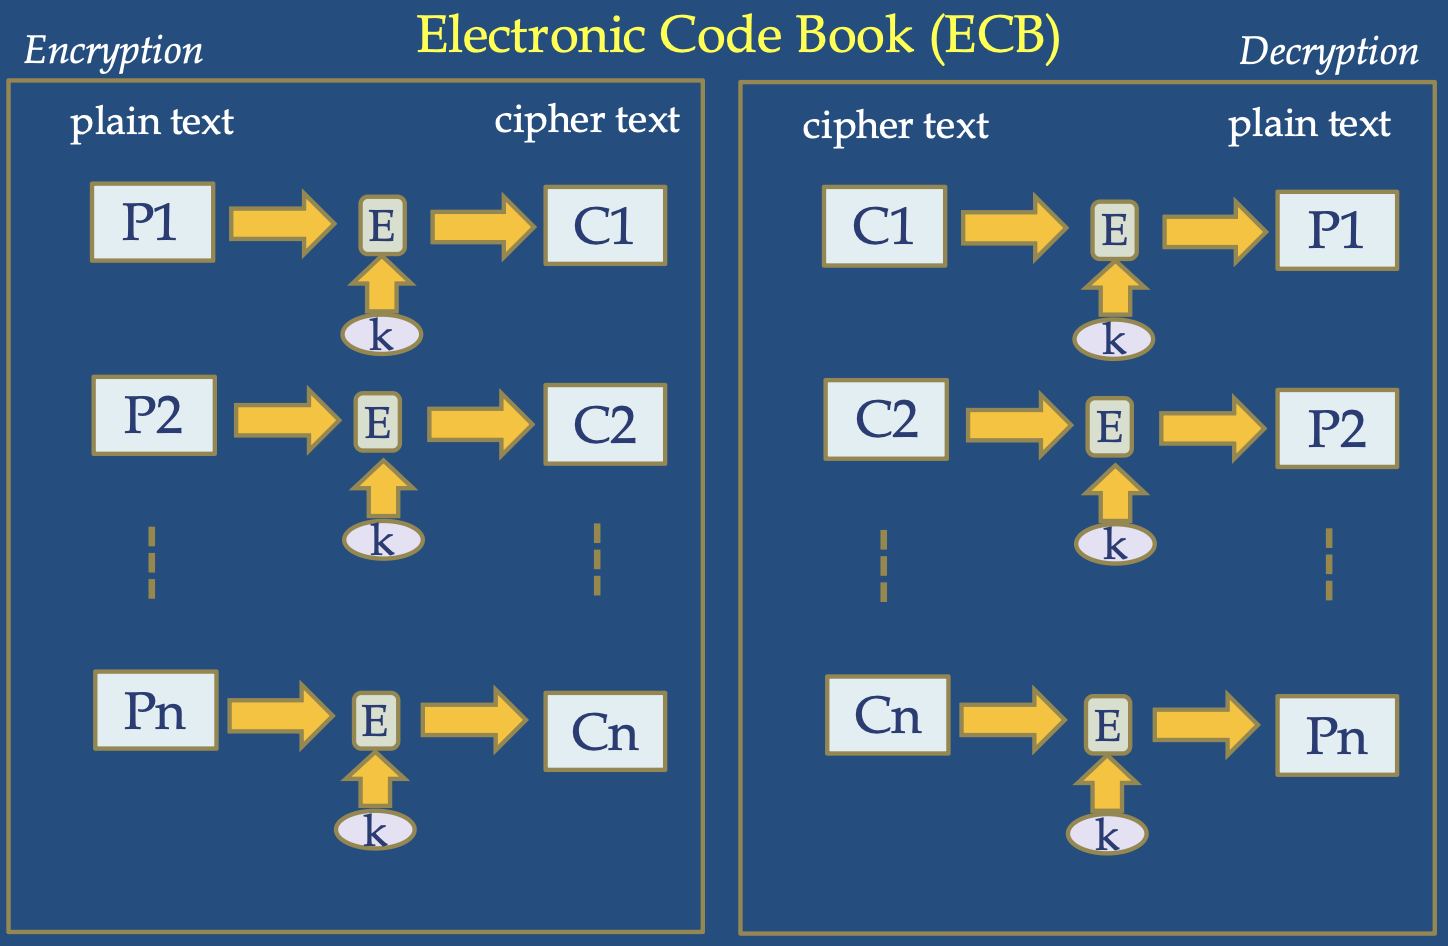
\includegraphics[width=\linewidth]{assets/Screenshot 2026-01-31 at 16.15.19.png}
        \caption{Electronic Code Book (ECB)}\label{fig:ecb}
    \end{subfigure}
    \begin{subfigure}{0.45\linewidth}
        \centering
        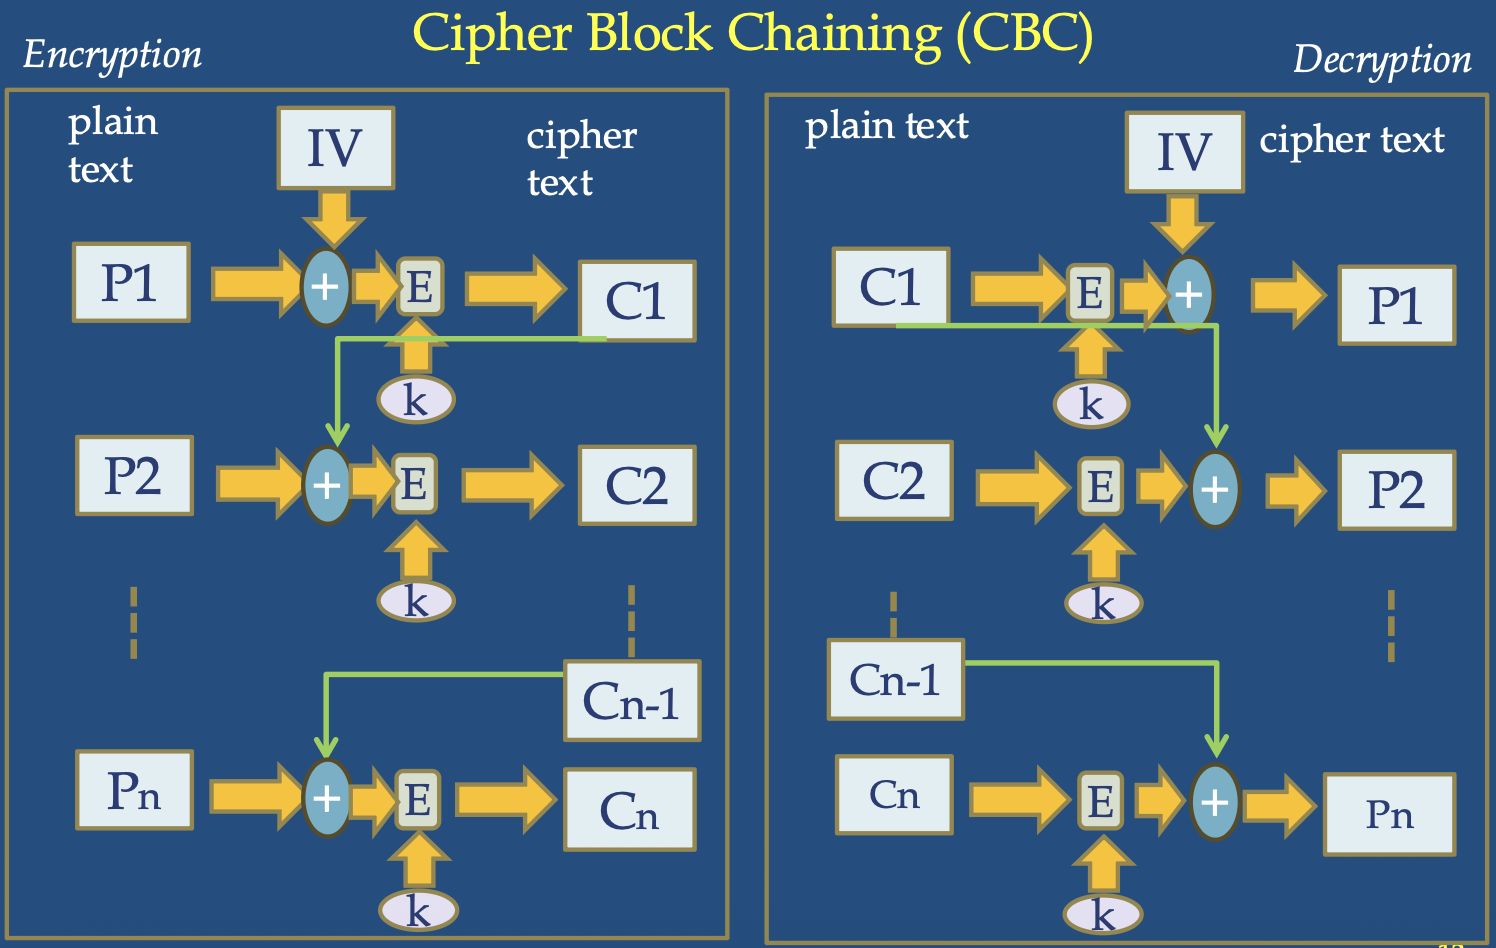
\includegraphics[width=\linewidth]{assets/Screenshot 2026-01-31 at 16.15.37.png}
        \caption{Cipher Block Chaining (CBC)}\label{fig:cbc}
    \end{subfigure}
    \caption{Algoritmi di crittografia a blocchi}\label{fig:block}
\end{figure}

%
\section{Distribuzione Chiavi e PKI}
%
\paragraph{Il problema della scalabilità}
\begin{itemize}
    \item \textbf{Simmetrico}: In un gruppo di utenti, il numero di chiavi necessarie cresce esponenzialmente ($N(N-1)/2$). Con 10 utenti servono 45 chiavi.
    \item \textbf{Asimmetrico}: Scala linearmente ($2N$). Con 10 utenti servono 20 chiavi.
\end{itemize}

%
\paragraph{Key Agreement: Diffie-Hellman} Permette a due parti (Alice e Bob) di concordare una chiave segreta comune comunicando su un canale pubblico insicuro.
\begin{enumerate}
    \item Si concordano due numeri pubblici: $p$ (primo) e $g$ (generatore);
    \item Alice sceglie un segreto $a$ e calcola $A = g^a \mod p$;
    \item Bob sceglie un segreto $b$ e calcola $B = g^b \mod p$;
    \item Si scambiano $A$ e $B$;
    \item Entrambi calcolano il segreto condiviso $S$: Alice fa $B^a \mod p$ e Bob fa $ A^b \mod p$. Il risultato è indentico.
\end{enumerate}

%
\paragraph{Public Key Infrastructure (PKI)} Per gestire le chiavi pubbliche in modo sicuro e associarle alle identità, si usa la PKI basata su terze parti fidate (TTP).
\begin{itemize}
    \item \textbf{Certificato X.509}: Lega una chiave pubblica a un soggetto (es. \verb|www.polito.it|). Contiene emittente, validità, algoritmo di firma e la firma della Certification Authority (CA);
    \item \textbf{Validità}: I certificati hanno una scadenza e possono essere revocati prima del tempo (es. se la chiave privata è compromessa);
    \item \textbf{Verifica Revoca}: Si usa la CRL (lista certificati revocati) o il protocollo OCSP (verifica online in tempo reale).
\end{itemize}

%
\section{Crittografia Ibrida e Integrità}
I sistemi moderni combinano le tecniche per efficienza e sicurezza.
%
\paragraph{Sistema misto (Hybrid)} La crittografia asimmetrica è lenta, quella simmetrica è veloce.
\begin{enumerate}
    \item Si usa l'algoritmo asimmetrico solo per scambiare in sicurezza una chiave simmetrica temporanea ($K_s$);
    \item Si usa l'algoritmo simmetrico (con la chiave $K_s$ appena scambiata) per cifrare l'effettivo traffico dati;
\end{enumerate}

%
\subsection{Hashing e Integrità} Per garantire che un messaggio non sia stato alterato, si usano funzioni di \emph{Digest} o \emph{Hash}.
%
\paragraph{Proprietà} Veloci da calcolare, impossibili da invertire, resistenti alle collisioni (due input diversi non devono produrre lo stesso hash).
%
\paragraph{Algoritmi di Hashing}
Tra i più utilizzati troviamo:
\begin{itemize}
    \item \textbf{MD5}: Digest 128 bit (RFC-1321);
    \item \textbf{SHA-1}: Digest 160 bit, \emph{debole};
    \item \textbf{SHA-2}: Digest 224-512 bit, \emph{forte};
    \item \textbf{SHA-3}: Standard recente (FIPS 202), \emph{molto forte}.
\end{itemize}

%
\section{Riepilogo Applicazioni di Sicurezza}
\begin{itemize}
    \item \textbf{Confidenzialità}: Dati illeggibili a terzi (AES);
    \item \textbf{Integrità}: Rilevamento modifiche ai dati (Hash SHA-256/SHA-3);
    \item \textbf{Autenticazione}: Verifica dell'identità (HMAC, Firma Digitale);
    \item \textbf{Non ripudio}: Il mittente non può negare di aver inviato il messaggio (Firma Digitale + PKI).
\end{itemize}